%%

\documentclass[final]{siamltex}
\usepackage{epsfig}
\usepackage{geometry}
\usepackage{color}
\usepackage{amsmath}
\usepackage{graphicx}
\usepackage{subfig}
\usepackage{amscd}
\usepackage{amsfonts, amssymb,mathrsfs}
% definitions used by included articles, reproduced here for
% educational benefit, and to minimize alterations needed to be made
% in developing this sample file.

\newcommand{\pe}{\psi}
\def\d{\delta}
\def\ds{\displaystyle}
\def\e{{\epsilon}}
\def\eb{\bar{\eta}}
\def\enorm#1{\|#1\|_2}
\def\Fp{F^\prime}
\def\fishpack{{FISHPACK}}
\def\fortran{{FORTRAN}}
\def\gmres{{GMRES}}
\def\gmresm{{\rm GMRES($m$)}}
\def\Kc{{\cal K}}
\def\norm#1{\|#1\|}
\def\wb{{\bar w}}
\def\zb{{\bar z}}

% some definitions of bold math italics to make typing easier.
% They are used in the corollary.

\def\bfE{\mbox{\boldmath$E$}}
\def\bfG{\mbox{\boldmath$G$}}

% My commands and macros (comment out if you don't want them)
\def \vec#1{{\bf{#1}}}
\def\pd#1#2{\dfrac{\partial #1}{\partial #2}}
\def \mat#1{\underline{\underline{#1}}}
\def \mylim#1#2{\lim_{#1 \rightarrow #2}}
\newcommand{\bi}{\begin{itemize}}
\newcommand{\ei}{\end{itemize}}
\newcommand{\func}{\mathcal{F}}
\newtheorem{thm}{Theorem}
\newtheorem{cor}[thm]{Corollary}
\newtheorem{lem}[thm]{Lemma}

\title{A Finite-Volume Approach to Black-Scholes Formula \thanks{Submitted for Math 250 Final Project, April 25, 2015}}

% The thanks line in the title should be filled in if there is
% any support acknowledgement for the overall work to be included
% This \thanks is also used for the received by date info, but
% authors are not expected to provide this.

\author{Sheng Xu
\thanks{Department of Mathematics, 503 Boston Ave, Tufts University,
Medford, MA 02155. {\it email:} {\tt
sheng.xu@tufts.edu}  } }


\begin{document}

\maketitle

%%%%%% ABSTRACT %%%%%%%%%%%%%%%%%%%%%%%%%%%%%%%%%%%%%%%%%%%%%%%%

%%%%%%%%%%%%%%%%%%%%%%%%%%%%%%%%%%%%%%%%%%%%%%%%%%%%%%%%%%%%

\begin{keywords}
Nonlinear PDEs, Finite-Volumn Method, Black-Scholes Formula, European Option, Option Pricing
\end{keywords}

\pagestyle{myheadings}
\thispagestyle{plain}
\markboth{\sc Xu, A Finite-Volume Approach to Black-Scholes Formula}{\sc}

%%%%%%%%%%%%%%%%%%%%%%%%%%%%%%%%%%%%%%%%%%%%%%%%%%%%%%%%%
%% Intro %%
%%%%%%%%%%%%%%%%%%%%%%%%%%%%%%%%%%%%%%%%%%%%%%%%%%%%%%%%%

\begin{abstract}
	Option Pricing problems during investment projects are mostly solved by the simulation-based methods, the lattice method and finite-difference method(FDM). There are also papers implies the successful application of the finite-element method(FEM), usually combined with techniques in FDM.\\
	In this paper, we investigated the application of the finite-volume method to the Black-Scholes Model and provide a detail scheme for pratical implementations. A modified finite-volume methhod is introduced as a numerical simulation of European Option Pricing. Detailed derivation process of the method is developed and numerical results ares provided. The numerical results are compared with Matlab built-in solver and show a good performance of the method. 
	
\end{abstract}

\section{Introduction} 
An option is a financial derivative that represents a contract sold by one party (the option writer) to another party (the option holder). The contract offers the buyer the right, but not the obligation, to buy (call) or sell (put) a security or other financial asset at an agreed-upon price (the strike price) during a certain period of time or on a specific date (exercise date)\cite{JohnHull}.\\

Black-Scholes(BS) Model\cite{BS} is one of the most commonly employed model based on partial difference equations, which provides an exact closed form solutions for financial derivatives. The equation is stated as: 
\begin{equation}
\frac{\partial V}{\partial t}+rS \frac{\partial V}{\partial S}+\frac{1}{2} \sigma ^2 S^2 \frac{\partial ^2 V}{\partial S ^2}-rV=0;
\end{equation}
where S is a real asset value, $0 \leq S \leq \infty$, V is the (real) option price, r is the risk-free rate, t is the time since the option was
issued, $0 \leq t \leq T$ , and $\sigma$ is the real asset volatility. This equation is a backward moving equation, i.e. it is solved from
the future to the present time.

For an European call option, the time condition becomes a final condition because its value is known at the maturity date
t = T and it is defined as its intrinsic value by:
\begin{equation}
V(S, T ) = max(S - K, 0), \forall S;
\end{equation}

For an European put option, the time condition becomes a final condition because its value is known at the maturity date
t = T and it is defined as its intrinsic value by:
\begin{equation}
V(S, T ) = max(K - S, 0), \forall S;
\end{equation}

This model has been mostly solved by the latice method\cite{lattice1,lattice2}, the finite-difference method(FDM)\cite{lattice2,FDM1} and simulation methods\cite{longstaff2001valuing,monteC1}. There are also papers applying finite-element method(FEM) to BS Model\cite{FEM1,FEM2}, suggesting good convergence. It is now known that the BS formula can be transformed into heat equation\cite{FEM1}:
\begin{equation}
\frac{\partial u}{\partial t} - \frac{\partial^2 u}{\partial \chi^2} = 0;
\end{equation} 

This offers a solid theoretical foundation to solve BS formula with FDM, FEM as well as finite-volume method(FVM)\cite{patankar1980numerical}. The finite volume method (FVM) is a method for representing and evaluating partial differential equations. Similar to the finite difference method or finite element method, values are calculated at discrete places on a meshed geometry. "Finite volume" refers to the small volume surrounding each node point on a mesh\cite{patankar1980numerical,leveque2002FVM}. In the finite volume method, volume integrals in a partial differential equation that contain a divergence term are converted to surface integrals, using the divergence theorem. One advantage of the finite volume method is that it is easily formulated to allow for non-uniform meshes\cite{versteeg2007FVM}. This is vital for pricing options with Black-Scholes Model. While the range of the asset price is quite wide, the values of options only change dramatically near the "current value" of asset value\cite{JohnHull}.\\

The finite-volume method is rarely studied with BS model. However, it is important to study other methods to numerically deal with this equation more quickly. Still, there are extreme conditions, mainly "smiles"\cite{JohnHull}, when the exact solution lose its accuracy and numerical results is extremely useful. In 2004, Wang\cite{wang2004FVM} introduced a method based on a fitted finite volume spatial discretization and an implicit time stepping technique. In this paper, we investigated the application of a finite-volume method to the Black-Scholes Model and provide a detail scheme for pratical implementations. A modified finite-volume methhod is introduced as a numerical simulation of European Option Pricing. Detailed derivation process of the method is developed and numerical results is provided. The numerical results are compared with Matlab built-in solver and show a good performance of the method.\\ 
%%%%%%%%%% MHD Equations &&&&&&&&&&&&&&&&&&&&&&&&&&&&&&&&&&&&&&&&&&&&


\section{Discretization of BS Model with FVM}
In section 1, we introduced the Black-Scholes Model and describe the parameters. It is known that we know a strike at time $t=T$ and want to calculate the price at time $0 \leq t<T$. To deal with the problem, we define $\tau = T-t$ and transform the formula into:
\begin{equation}
\frac{\partial V}{\partial \tau}=rS \frac{\partial V}{\partial S}+\frac{1}{2} \sigma ^2 S^2 \frac{\partial ^2 V}{\partial S ^2}-rV;
\label{BS_Formula}
\end{equation}
where S is a real asset value, $0 \leq S \leq \infty$, V is the (real) option price, r is the risk-free rate, $\tau$ is the time before the option is
exercised, $0 \leq \tau \leq T$ , and $\sigma$ is the real asset volatility.  \\

For the first step, we show how to transform the Black-Scholes Formula into diffustion equation\cite{FEM1}. Let:
\begin{equation}
\begin{split}
&\chi=ln \frac{S}{K},\\
&\gamma = \frac{\sigma ^2}{2}(T-t),\\
&\upsilon(\chi,\gamma)=\frac{1}{K}V(S,t)e^{\frac{1}{2}(k_1-1)\chi+\frac{1}{4}(K_1+1)^2 \gamma};
\end{split}
\end{equation}
where $k_1=\frac{2r}{\sigma^2}$. Thus, we will have: $\frac{\partial \upsilon}{\partial \gamma}-\frac{\partial ^2 \upsilon}{\partial \chi ^2}=0$.

We then integrate the equation (\ref{BS_Formula}) on a divided domain $ A_i$ $ \times$ $T_n$ = $[S_{i-\frac{1}{2}},S_{i+\frac{1}{2}}]$ $\times$ $[\tau_n , \tau_{n+1}]$, where $S_{i-\frac{1}{2}}= \frac{1}{2} (S_{i-1}+S_{i})$; $S_{i+\frac{1}{2}}=\frac{1}{2} (S_{i}+S_{i+1})$. \\
Let $\|T_n\|=$ $\Delta \tau=\tau_{n+1}-\tau_{n}$; $\|A_i\|= S_{i+\frac{1}{2}}-S_{i-\frac{1}{2}}= \frac{1}{2}(S_{i+1}-S_{i-1})$; $V_n^i=V(S _i, \tau _n)$. This will give us the formula:
\begin{equation}
\int _{A_i} V_i^{n+1}- V_i^{n}= \Delta \tau (\int _{A_i} rS \frac{\partial V}{\partial S}+ \int _{A_i} \frac{1}{2} \sigma ^2 S^2 \frac{\partial ^2 V}{\partial S ^2}- \|A_i\| rV);
\label{Int}
\end{equation}
The left-hand side gives:
\begin{equation}
\int _{A_i} V_i^{n+1}- V_i^{n}=\|A_i\|(V_i^{n+1}- V_i^{n});
\label{Int_L1}
\end{equation}
For the right-hand side, using Approximation we have:
\begin{equation}
\begin{split}
\int _{A_i} rS \frac{\partial V}{\partial S}
&\approx rS_i[V^{n+1}_{i+\frac{1}{2}}-V^{n+1}_{i-\frac{1}{2}}]\\
&\approx \frac{1}{2}rS_i[V^{n+1}_{i+1}-V^{n+1}_{i-1}];
\end{split}
\label{Int_R1}
\end{equation}
And:
\begin{equation}
\begin{split}
\int _{A_i} \frac{1}{2} \sigma ^2 S^2 \frac{\partial ^2 V}{\partial S ^2}
&\approx \frac{1}{2} \sigma ^2 S_i^2 [(V_S)_{i+\frac{1}{2}}
-(V_S)_{i-\frac{1}{2}}] \\
&\approx \frac{1}{2} \sigma ^2 S_i^2 (\frac{V^{n+1}_{i+1}-V^{n+1}_i}{S_{i+1}-S_i} - \frac{V^{n+1}_{i}-V^{n+1}_{i-1}}{S_{i}-S_{i-1}});
\end{split}
\label{Int_R2}
\end{equation}
Now let's assemble (\ref{Int_L1}) (\ref{Int_R1}) (\ref{Int_R2}) into (\ref{Int}) and using the implicit scheme simlar to FDM:
\begin{equation}
\begin{split}
\|A_i\|(V_i^{n+1}- V_i^{n}) \approx  \Delta \tau &(\frac{1}{2}rS_i[V^{n+1}_{i+1}-V^{n+1}_{i-1}]\\
& +\frac{1}{2} \sigma ^2 S_i^2 [\frac{V^{n+1}_{i+1}-V^{n+1}_i}{S_{i+1}-S_i} 
- \frac{V^{n+1}_{i}-V^{n+1}_{i-1}}{S_{i}-S_{i-1}}] \\
& - \|A_i\| rV_i^{n+1});
\end{split}
\label{FVM_BS}
\end{equation}

This gives an implicit formula of $V^n$ and $V^{n+1}$.
\begin{equation}
V_i^n \approx \alpha _{i-1} V_{i-1}^{n+1} + \alpha _{i} V_{i}^{n+1} + \alpha _{i+1} V_{i+1}^{n+1};
\label{FVM_Split}
\end{equation}
where 
\begin{equation}
\begin{split}
& \alpha_{i-1}  =  -\frac {\sigma^2 S_i^2 \Delta \tau}{(S_{i+1} -S_{i-1}) (S_{i}-S_{i-1})} + \frac{S_i r \Delta \tau} {S_{i+1}-S_{i-1}},\\
& \alpha_{i}  = 1 - \frac {\sigma^2 S_i^2 \Delta \tau}{(S_{i}-S_{i-1}) (S_{i+1}-S_i)} + r \Delta \tau,\\
& \alpha_{i+1}  = -\frac {\sigma^2 S_i^2 \Delta \tau}{(S_{i+1} -S_{i-1}) (S_{i+1}-S_i)} - \frac{S_i r \Delta \tau} {S_{i+1}-S_{i-1}};
\end{split}
\label{FVM_Coef}
\end{equation}

\section{Numerical Results}
In this part, we discuss our result of the implementation of the algrithm. Here, We set our parameters as:
\begin{align*}
\sigma = 0.4,
r = 0.05,
K = 100,
T = 1,
n=4;
\end{align*}
According to the behavior of the price of options, we input an S like this:
\begin{align*}
\begin{split}
S =  K/100*&[0:20:60 \quad 61:4:89 \quad 90:0.8:110 \quad \\
 & \quad 111:4:139 \quad 140:20:200 \quad 300 \quad 500 \quad 1000 \quad 5000];
\end{split}
\end{align*}
$2^{(n-1)}-1$ points are added into each two points in S, dividing the intervals in S into $2^n$ subintervals. We also descritize the time into $365*2^{n-1}*T$ sub intervals.Note according the nature that the change of value for $S \notin [80, 100]$ is slow, so we use bigger intervals outside [80, 100]. The figures of n=4 are on Page 8~11. We briefly introduce the figures: 

Figure 3.1-3.4 gives the result of a European call option; Figure 3.5-3.8 gives the result of a European put option. Here we set n=4. The error of European call option is 0.0022 on $S\in [80,120]$. The error of European put option is 0.0021 on $S\in [80,120]$. 

We now numerically study the relation of error and size of meshes $\sigma = 0.4;
r = 0.05;
K = 100;
T = 1$; type="call": 
\begin{table}[h!]
	\centering
	{\small
		\begin{tabular}{|c|c|c|c|c|c|c|}
			
			\hline
			
			$\Delta \tau$ &$\Delta S$ for $S \in [80,120]$&FVM Run-Time &Matlab Fcn Run-Time &Max Error on $S\in[80,120]$\\
			
			\hline
			
			$\frac{1}{365}$&0.4&0.021&0.220&0.0276\\
			
			$\frac{1}{365}$&0.2&0.101&0.311&0.0122\\
			
			$\frac{1}{365}$&0.1&0.643&0.703&0.0073\\
			
			\hline
			
			$\frac{1}{730}$&0.4&0.038&0.202&0.0249\\
			
			$\frac{1}{730}$&0.2&0.180&0.362&0.0086\\
			
			$\frac{1}{730}$&0.1&1.000&0.688&0.0042\\
			
			\hline
			
			$\frac{1}{1460}$&0.4&0.077&0.222&0.0241\\
			
			$\frac{1}{1460}$&0.2&0.366&0.373&0.0073\\
			
			$\frac{1}{1460}$&0.1&1.744&0.658&0.0028\\
			
			\hline
			
			
			$\frac{1}{2920}$&0.4&0.200&0.292&0.0237\\
			
			$\frac{1}{2920}$&0.2&0.679&0.380&0.0066\\
			
			$\frac{1}{2920}$&0.1&4.055&0.696&0.0022\\
			
			\hline
			
		\end{tabular}
	}
	
	\caption{Running Time and Error according to $\Delta S$ and $\Delta \tau$}
	\label{tearingunif}
\end{table}

We see that the running time of FVM is increasing by $\frac{1}{\Delta \tau}$ and $\frac{1}{\Delta S^2}$ respectively. We discuss the truncation error in the next section.

\begin{figure}[H]
	\centering
	 
		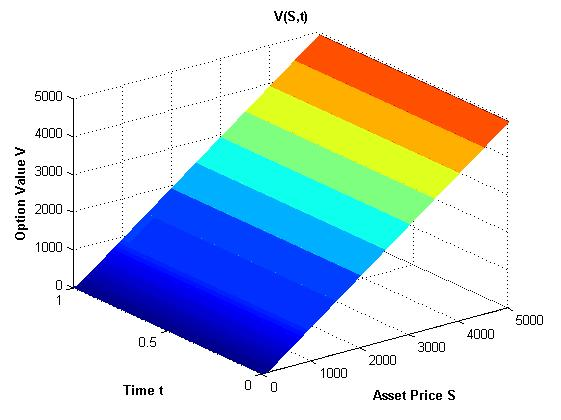
\includegraphics[width=0.8\textwidth]{European_call_all}
		\caption{European Call Option: S $\times $ T= [0,5000] $\times $ [0,1]}
	
		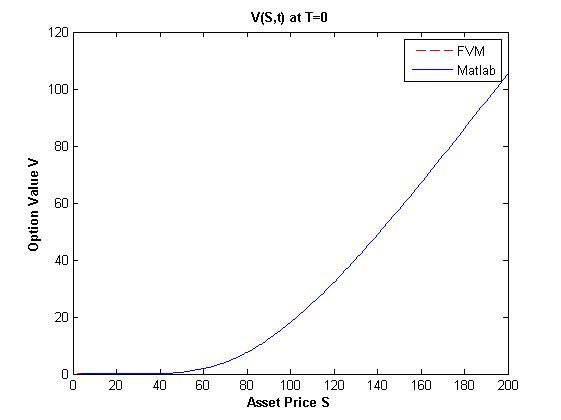
\includegraphics[width=0.8\textwidth]{European_call_Final_all}
		\caption{European Call Option: S $\times $ T= [0,200] $\times $ [0,1]}

		\label{European_call_all}	
\end{figure}

\begin{figure}[H]
	\centering
	
	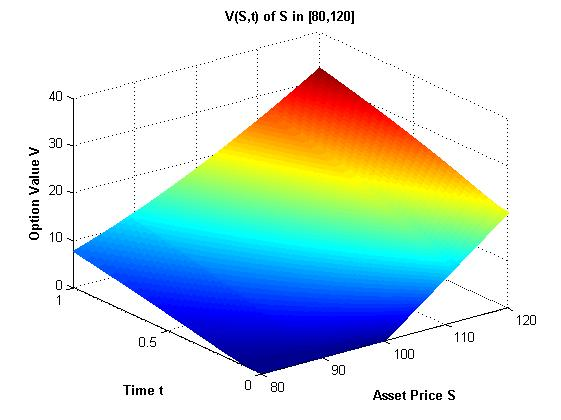
\includegraphics[width=0.8\textwidth]{European_call_main}
	\caption{European Call Option: S $\times $ T= [80,120] $\times $ [0,1]}
	
	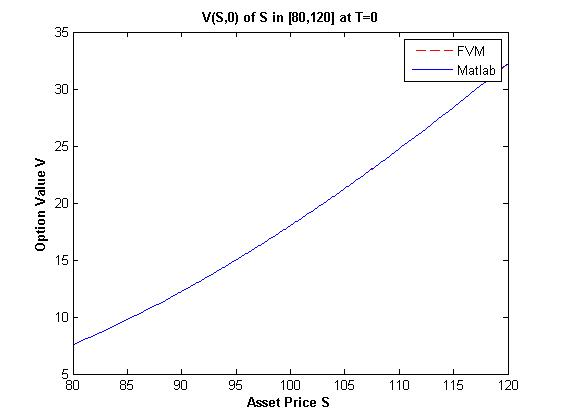
\includegraphics[width=0.8\textwidth]{European_call_Final20}
	\caption{European Call Option: S $\times $ T= [80,120] $\times $ [0,1]}
	\label{European_call_main}	
\end{figure}
%\includegraphics [width = 5cm] {European_call_100_1_0.05_0.4_al.jpg}
\begin{figure}[H]
	\centering
	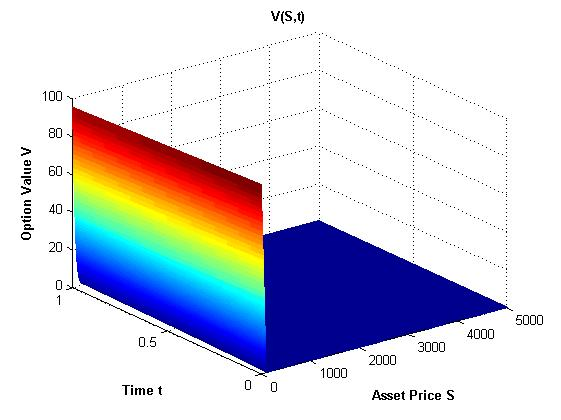
\includegraphics[width=0.8\textwidth]{European_put_all}
	\caption{European Put Option: S $\times $ T= [0,5000] $\times $ [0,1]}
	
	\includegraphics[width=0.8\textwidth]{European_Put_Final_all}
	\caption{European Put Option Compared with Matlab: S $\times $ T= [0,200] $\times $ {1}}
	\label{European_put_all}	
\end{figure}

\begin{figure}[H]
	\centering
	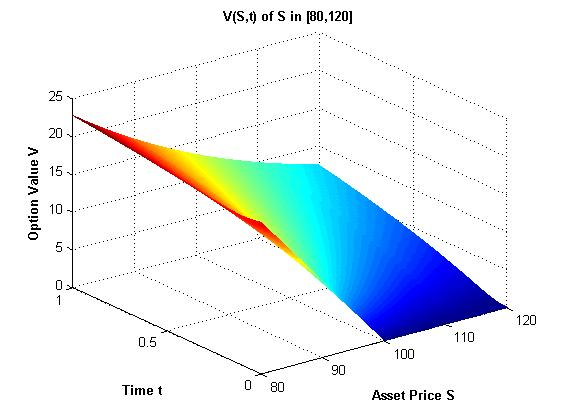
\includegraphics[width=0.8\textwidth]{European_put_main}
	\caption{European Put Option: S $\times $ T= [80,120] $\times $ [0,1]}
	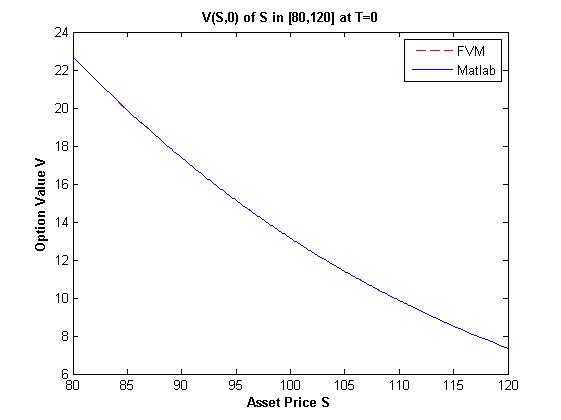
\includegraphics[width=0.8\textwidth]{European_put_Final20}
	\caption{European Put Option Compared with Matlab: S $\times $ T= [80,120] $\times $ {1}}
	\label{European_put_main}	
\end{figure}

\section{Error Estimate and Stability}
In previous sections, we have:
\begin{equation}
\begin{split}
\|A_i\|(V_i^{n+1}- V_i^{n}) \approx  \Delta \tau &(\frac{1}{2}rS_i[V^{n+1}_{i+1}-V^{n+1}_{i-1}]\\
& +\frac{1}{2} \sigma ^2 S_i^2 [\frac{V^{n+1}_{i+1}-V^{n+1}_i}{S_{i+1}-S_i} 
- \frac{V^{n+1}_{i}-V^{n+1}_{i-1}}{S_{i}-S_{i-1}}] \\
& - \|A_i\| rV_i^{n+1});
\end{split}
\tag{\ref{FVM_BS}}
\end{equation}

We modify the equation (\ref{FVM_BS}) a little bit to match the form of equation (\ref{BS_Formula}) and write $\varepsilon$ as truncation error:
\begin{equation}
\begin{split}
\varepsilon = & \frac{V_i^{n+1}- V_i^{n}}{\Delta \tau} -  \frac{rS_i}{2\|A_i\|}[V^{n+1}_{i+1}-V^{n+1}_{i-1}]\\
&-\frac{\sigma^2 S_i^2}{2\|A_i\|}[\frac{V^{n+1}_{i+1}-V^{n+1}_i}{S_{i+1}-S_i} 
- \frac{V^{n+1}_{i}-V^{n+1}_{i-1}}{S_{i}-S_{i-1}}]+ rV_i^{n+1};
\end{split}
\label{Truncation}
\end{equation}
We start from here and employ the Taylor Expansion to the third power (assuming uniform meshes $\Delta \tau = \tau_{n+1}-\tau_{n}$, $\Delta S=\|A_i\|=S_{i+1}-S_i$):
\begin{equation}
\begin{split}
\frac{V_i^{n+1}- V_i^{n}}{\Delta \tau} &= \frac{V_i^{n+1}-(V_i^{n+1}- V_{i_\tau}^{n+1}\Delta \tau+\frac{1}{2}V_{i_{\tau \tau}}^{n+1}\Delta \tau^2-K_1\Delta \tau^3)}{\Delta \tau}\\ 
&=V_{i_\tau}^{n+1}-\frac{1}{2}V_{i_{\tau \tau}}^{n+1}\Delta \tau + K_1 \Delta \tau^2;
\end{split}
\label{Truncation1}
\end{equation}

\begin{equation}
\begin{split}
\frac{rS_i}{2\|A_i\|}[V^{n+1}_{i+1}-V^{n+1}_{i-1}]&= \frac{rS_i}{2\|A_i\|}[(V^{n+1}_{i}+ V^{n+1}_{i_{S}}\Delta S+\frac{1}{2}V^{n+1}_{i_{SS}}\Delta S^2+ K_{2a} \Delta S^3 )\\ 
&\quad -(V^{n+1}_{i}- V^{n+1}_{i_{S}}\Delta S+\frac{1}{2}V^{n+1}_{i_{SS}}\Delta S^2- K_{2b} \Delta S^3 )]\\
&=rS_iV^{n+1}_{i_{S}}+ K_2 \Delta S^2;
\end{split}
\label{Truncation2}
\end{equation}
\begin{equation}
\begin{split}
&\frac{\sigma^2 S_i^2}{2\|A_i\|}[\frac{V^{n+1}_{i+1}-V^{n+1}_i}{S_{i+1}-S_i}- \frac{V^{n+1}_{i}-V^{n+1}_{i-1}}{S_{i}-S_{i-1}}]\\
&=
\frac{\sigma^2 S_i^2}{2\Delta S} [\frac{(V^{n+1}_{i}+ V^{n+1}_{i_{S}}\Delta S+\frac{1}{2}V^{n+1}_{i_{SS}}\Delta S^2+ \frac{1}{6}V^{n+1}_{i_{SSS}}\Delta S^3+K_{3a} \Delta S^4)-V^{n+1}_i}{\Delta S}\\
&\quad -\frac{V^{n+1}_i-(V^{n+1}_{i}- V^{n+1}_{i_{S}}\Delta S+\frac{1}{2}V^{n+1}_{i_{SS}}\Delta S^2-\frac{1}{6}V^{n+1}_{i_{SSS}}\Delta S^3 +K_{3b} \Delta S^4)}{\Delta S}]\\
&= \frac{\sigma^2 S_i^2}{2}V^{n+1}_{i_{SS}}+K_3\Delta S^2;
\end{split}
\label{Truncation3}
\end{equation}
where $K_2=\frac{rS_i}{2}[K_{2a}+K_{2b}]$; $K_3=\frac{\sigma^2 S_i^2}{2}[K_{3a}+K_{3b}]$.

Therefore, according to (\ref{Truncation}) with (\ref{Truncation1}) (\ref{Truncation2}) (\ref{Truncation3}), we have:
\begin{equation}
\begin{split}
	\varepsilon = V_{i_\tau}^{n+1}-\frac{1}{2}V_{i_{\tau \tau}}^{n+1}\Delta \tau + K_1 \Delta \tau^2-rS_iV^{n+1}_{i_{S}} - K_2 \Delta S^2
	- \frac{\sigma^2 S_i^2}{2}V^{n+1}_{i_{SS}}-K_3\Delta S^2+ rV_i^{n+1};
\end{split}
\label{TruncationSumUp}
\end{equation}

Recall from (\ref{BS_Formula}) we have:
\begin{equation}
\begin{split}
V_{i_\tau}^{n+1}=rS_iV^{n+1}_{i_{S}} 
+ \frac{\sigma^2 S_i^2}{2}V^{n+1}_{i_{SS}}- rV_i^{n+1};
\end{split}
\label{TruncationCancelOut}
\end{equation}
This will help us cancel out the $V_{i_\tau}^{n+1}$, $rS_iV^{n+1}_{i_{S}} $, 
$ \frac{\sigma^2 S_i^2}{2}V^{n+1}_{i_{SS}}$, $rV_i^{n+1}$ terms, leaving:
\begin{equation}
\begin{split}
\varepsilon = -\frac{1}{2}V_{i_{\tau \tau}}^{n+1}\Delta \tau + K_1 \Delta \tau^2 - K_2 \Delta S^2-K_3\Delta S^2;
\end{split}
\label{TruncationResult}
\end{equation}

So the truncation error is $O(\Delta \tau, \Delta S^2)$.

Next, we analize the stability. Again, recall (\ref{FVM_Split}):
\begin{equation}
V_k^n \approx \alpha _{k-1} V_{k-1}^{n+1} + \alpha _k V_{k}^{n+1} + \alpha _{k+1} V_{k+1}^{n+1};
\tag{\ref{FVM_Split}}
\end{equation}
where with uniform meshes:
\begin{equation}
\begin{split}
& \alpha_{k-1}  =  -\frac {\sigma^2 S_k^2 \Delta \tau}{2\Delta S^2} + \frac{S_k r \Delta \tau} {2\Delta S};\\
& \alpha_{k}  = 1 - \frac {\sigma^2 S_k^2 \Delta \tau}{\Delta S^2} + r \Delta \tau;\\
& \alpha_{k+1}  = -\frac {\sigma^2 S_k^2 \Delta \tau}{2\Delta S^2} - \frac{S_k r \Delta \tau} {2\Delta S};
\end{split}
\end{equation}

Writing $V_k^n=\hat{e}_n^{(j)} e^{ijk\Delta S}$, $V_k^{n+1}=\hat{e}_{n+1}^{(j)} e^{ijk\Delta S}$, then we have:
\begin{equation}
\begin{split}
\hat{e}_n^{(j)} e^{ijk\Delta S} = \alpha _{k-1} \hat{e}_{n+1}^{(j)} e^{ij(k-1)\Delta S} + \alpha _k \hat{e}_{n+1}^{(j)} e^{ijk\Delta S} + \alpha _{k+1}\hat{e}_{n+1}^{(j)} e^{ij(k+1)\Delta S};
\end{split}
\end{equation}
\begin{equation}
\begin{split}
\hat{e}_n^{(j)}  = \alpha _{k-1} \hat{e}_{n+1}^{(j)} e^{-ij\Delta S} + \alpha _k \hat{e}_{n+1}^{(j)} + \alpha _{k+1}\hat{e}_{n+1}^{(j)} e^{ij\Delta S};
\end{split}
\end{equation}
We take in all coefficents:
\begin{equation}
\begin{split}
\hat{e}_n^{(j)}  = &[-\frac {\sigma^2 S_k^2 \Delta \tau}{2\Delta S^2} + \frac{S_k r \Delta \tau} {2\Delta S}] \hat{e}_{n+1}^{(j)} e^{-ij\Delta S} + [1 - \frac {\sigma^2 S_k^2 \Delta \tau}{\Delta S^2} + r \Delta \tau] \hat{e}_{n+1}^{(j)}\\ &+ [-\frac {\sigma^2 S_k^2 \Delta \tau}{2\Delta S^2}- \frac{S_k r \Delta \tau} {2\Delta S}]\hat{e}_{n+1}^{(j)} e^{ij\Delta S};
\end{split}
\end{equation}
Hence:
\begin{equation}
\begin{split}
\hat{e}_n^{(j)} = \hat{e}_{n+1}^{(j)}[1+\frac {\sigma^2 S_k^2 \Delta \tau}{\Delta S^2}(2-2cos(j\Delta S))+r\Delta \tau-i \frac{S_k r \Delta \tau} {\Delta S}sin(j\Delta S)]
\end{split}
\end{equation}
Since $|1+\frac {\sigma^2 S_k^2 \Delta \tau}{\Delta S^2}(2-2cos(j\Delta S))+r\Delta \tau-i \frac{S_k r \Delta \tau} {\Delta S}sin(j\Delta S)|\geq \sqrt{1 + r^2\Delta \tau^2}>1$, so the method is stable as $|\hat{e}_{n+1}^{(j)}|<|\hat{e}_{n}^{(j)}|$.

%%%%%%%%%%%%%%%%%%%%%%%%%%%%%%%%%%%%%%%%%%%%%%%%%%%%%%%%%
%% Conclusion %%
%%%%%%%%%%%%%%%%%%%%%%%%%%%%%%%%%%%%%%%%%%%%%%%%%%%%%%%%%
\section{Conclusion}
In this paper, we have described a Finite-Volume Method for option pricing using Black-Schole Model. We integrated the function on a small mesh $[S_{i-\frac{1}{2}},S_{i+\frac{1}{2}}]\times[\tau_{n},\tau_{n+1}]$ and generated the relation between the price of option at $t$ and $t+\Delta t$ in a discrete form:
\begin{equation*}
V_i^n \approx \alpha _{i-1} V_{i-1}^{n+1} + \alpha _{i} V_{i}^{n+1} + \alpha _{i+1} V_{i+1}^{n+1};
\end{equation*}
where 
\begin{equation*}
\begin{split}
& \alpha_{i-1}  =  -\frac {\sigma^2 S_i^2 \Delta \tau}{(S_{i+1} -S_{i-1}) (S_{i}-S_{i-1})} + \frac{S_i r \Delta \tau} {S_{i+1}-S_{i-1}};\\
& \alpha_{i}  = 1 - \frac {\sigma^2 S_i^2 \Delta \tau}{(S_{i}-S_{i-1}) (S_{i+1}-S_i)} + r \Delta \tau;\\
& \alpha_{i+1}  = -\frac {\sigma^2 S_i^2 \Delta \tau}{(S_{i+1} -S_{i-1}) (S_{i+1}-S_i)} - \frac{S_i r \Delta \tau} {S_{i+1}-S_{i-1}};
\end{split}
\end{equation*}

Then we applied the formula in Matlab and compare the numerical result of the method with the analytic solution of the Matlab built-in function. The result shows a high accuracy with $\Delta S = 0.1$ when $S\in [80,120]$, $\Delta \tau = \frac{1}{365*8}$ (about \$0.002 per share when $S \in [80,120]$). The running time of this mesh was about 8 time of that of the matlab built-in function. However, one could choose a bigger mesh and still got a good accuracy (less than \$0.01 per share) and reduce the runnning time close to or even less than that of the matlab built-in function.

We further studied the trunction error and stability of this method. The accuracy turned out to be $O(\Delta \tau, \Delta S^2)$ and the method is unconditionally stable. Both show the good feasibility of the method. For future study, we can try to apply numerical methods to solve equation(\ref{FVM_BS}) more efficiently.

%%%%%%%%%%%%%%%%%%%%%%%%%%%%%%%%%%%%%%%%%%%%%%%%%%%%%%%%%
%% References %%
%%%%%%%%%%%%%%%%%%%%%%%%%%%%%%%%%%%%%%%%%%%%%%%%%%%%%%%%%
\bibliographystyle{unsrt}	% or "siam", or "alpha", or "abbrv"
				% see other styles (.bst files) in
				% $TEXHOME/texmf/bibtex/bst
\nocite{*}		% list all refs in database, cited or not.
\bibliography{refs}		% bib database file refs.bib

\end{document}

